\documentclass[12pt,titlepage]{article}
\usepackage[spanish]{babel}
\usepackage[utf8]{inputenc}
\usepackage{amsfonts}
\usepackage{amsmath}
\usepackage{amssymb}
\usepackage{color}
\usepackage{graphicx} % para insertar imagenes
\usepackage{caratulaMetNum}
\usepackage{verbatim}
\usepackage{float}


\newcommand{\func}[2]{\texttt{#1}(#2)}
\newcommand{\funcFull}[2]{\texttt{#1}=#2}
\newcommand{\tab}{\hspace*{2em}}
\newcommand{\FOR}{\textbf{for }}
\newcommand{\END}{\textbf{end }}
\newcommand{\TO}{\textbf{ to }}
\newcommand{\IF}{\textbf{if }}
\newcommand{\WHILE}{\textbf{while }}
\newcommand{\THEN}{\textbf{then }}
\newcommand{\ELSE}{\textbf{else }}
\newcommand{\RET}{\textbf{return }}
\newcommand{\MOD}{\textbf{ \% }}
\newcommand{\OR}{\textbf{ or }}
\newcommand{\AND}{\textbf{ and }}
\newcommand{\tOde}[1]{\tab \small{O($#1$)}}
\newcommand{\Ode}[1]{O($#1$)}
\newcommand{\Thetade}[1]{{\small$\Theta$($#1$)}}
\newcommand{\Omegade}[1]{{\small$\Omega$($#1$)}}
\newcommand{\VSP}{\vspace*{3em}}
\newcommand{\pa}{\vspace{5mm}}
\newcommand{\e}[2]{\varepsilon  _{#1}({#2})}
\newcommand{\er}[2]{\varepsilon _{({#1})}^{({#2})}}
\newcommand{\ev}[1]{\varepsilon _{#1}}
\newcommand{\N}{\mathbb{N}}
\newenvironment{pseudo}{\begin{tabular}{p{11cm}l}}{\end{tabular}\VSP}


\newcommand{\gra}[1]{{\noindent\centering\includegraphics[width=14cm]{#1}}\\}

\begin{document}

\materia{Métodos Numéricos}
\titulo{Trabajo Práctico Nº2}
\subtitulo{Guerra lineal}
\integrante{Carla Livorno}{424/08}{carlalivorno@hotmail.com}
\integrante{Mariano De Sousa Bispo}{389/08}{marian\_sabianaa@hotmail.com}

\abstracto{
	bla bla bla bla bla bla bla bla bla bla bla bla
}

\palabraClave{Sistemas lineales}
\palabraClave{}
\palabraClave{}

\begin{titlepage}
\maketitle
\end{titlepage}
\tableofcontents
\newpage
	\begin{section}{Introducción teórica}	

\end{section}

	\newpage
	\begin{section}{Desarrollo}
	\begin{subsection}{Explicación}
		
	\end{subsection}
	\begin{subsection}{Implementación}
		La implementación esta divida en módulos que realizan tareas especificas, a continuación detallaremos cada uno de ellos.
		
		\begin{itemize}
			\item \underline{Módulo Parametrización:}\\
				Este módulo implementa las $tres$ parametrizaciones (uniforme, chord-length, centripeta) a partir de un conjunto de puntos de control.
			\item \underline{Módulo Polinomio:}\\
				Escribimos el módulo \texttt{Polinomio} que implementa un polinomio de grado $n$ con las siguientes operaciones:\\
				
				\begin{tabular}{rl}
					\texttt{Evaluar} & Evalua el polinomio en un valor recibido como parámetro.\\
					\texttt{Derivar} & Realiza la derivada primera del polinomio.\\
					\texttt{Ceros}   & Busca una raíz del polinomio usando bisección y el método de Newton.\\
				\end{tabular}\\
				EXPLICAR CON MAYOR DETALLES LAS OPERACIONES (COMO NEWTON)!!!!!!
		
			\item \underline{Módulo Spline:}\\
				Escribimos el módulo \texttt{Spline} que implementa un spline cúbico natural con las siguientes operaciones:\\
				
				\begin{tabular}{rl}
					\texttt{Evaluar} & Evalua la spline (el polinomio correspondiente) en un valor recibido como parámetro.\\
					\texttt{Polinomio} & Devuelve el polinomio requerido.\\
				\end{tabular}\\

			\item \underline{Módulo Curva:}\\
				El módulo \texttt{curva} implementa una curva parámetrica con las siguientes operaciones:\\
				
				\begin{tabular}{rl}
					\texttt{Evaluar} & Evalua la spline (el polinomio correspondiente) en un valor recibido como parámetro.\\
					\texttt{Polinomio} & Devuelve el $n-esimo$ polinomio (siendo $n$ el parámetro).\\
				\end{tabular}\\
		\end{itemize}
	\end{subsection}
\end{section}

	\newpage
	\begin{section}{Resultados}
	El siguiente gráfico se realizó para ajustar un parámetro ($epsilon$) del programa que sirve para generar las
	matrices mal condicionadas. Recordar que una matriz mal condicionada se construye a partir de un vector que 
	resulta en las filas de la misma y luego se le suma el $epsilon$ a los elementos de la diagonal para que quede 
	inversible.
	
	Con esta prueba esperamos ver que cuanto menor es el $epsilon$ mayor es el número de condición de la matriz
	 debido a que las filas están más cerca de ser linealmente dependientes y por ende la matriz más cerca de ser
	  singular.

	El gráfico muestra el número de condición de la matriz en función de su dimensión para los siguientes valores de
	$epsilon$: $1$, $1e^{-1}$, $1e^{-2}$, $1e^{-3}$, $1e^{-4}$, $1e^{-5}$ y $1e^{-6}$. Elegimos esos valores de
	$epsilon$ ya que para generarlos tenemos una variable $v$ ($unsigned\;int$) que itera por los múltiplos de $10$ 
	(empezando en $1$),	siendo $epsilon$ igual a $1.0/v$. El mayor múltiplo de $10$ que $v$ es capaz de almacenar es $1e^9$ 
	pero con $epsilon$ igual a $1e^{-7}$, $1e^{-8}$ y $1e^{-9}$ las matrices generadas quedaban singulares en muchas
	ocasiones, suponemos que eso se debe a que estos valores de $epsilon$ ya son despreciables ($cero$) y al sumarle 
	ese valor a la diagonal no conseguimos filas linealmente dependientes como queremos.
	
	Corrimos las pruebas para matrices de dimensión $2$ a dimensión $50$.
	El eje que corresponde al \texttt{número de condición} está en escala logarítmica para poder apreciar mejor los valores correspondientes dado que estos crecen exponencialmente.

	\begin{figure}[H]
	  \centering
		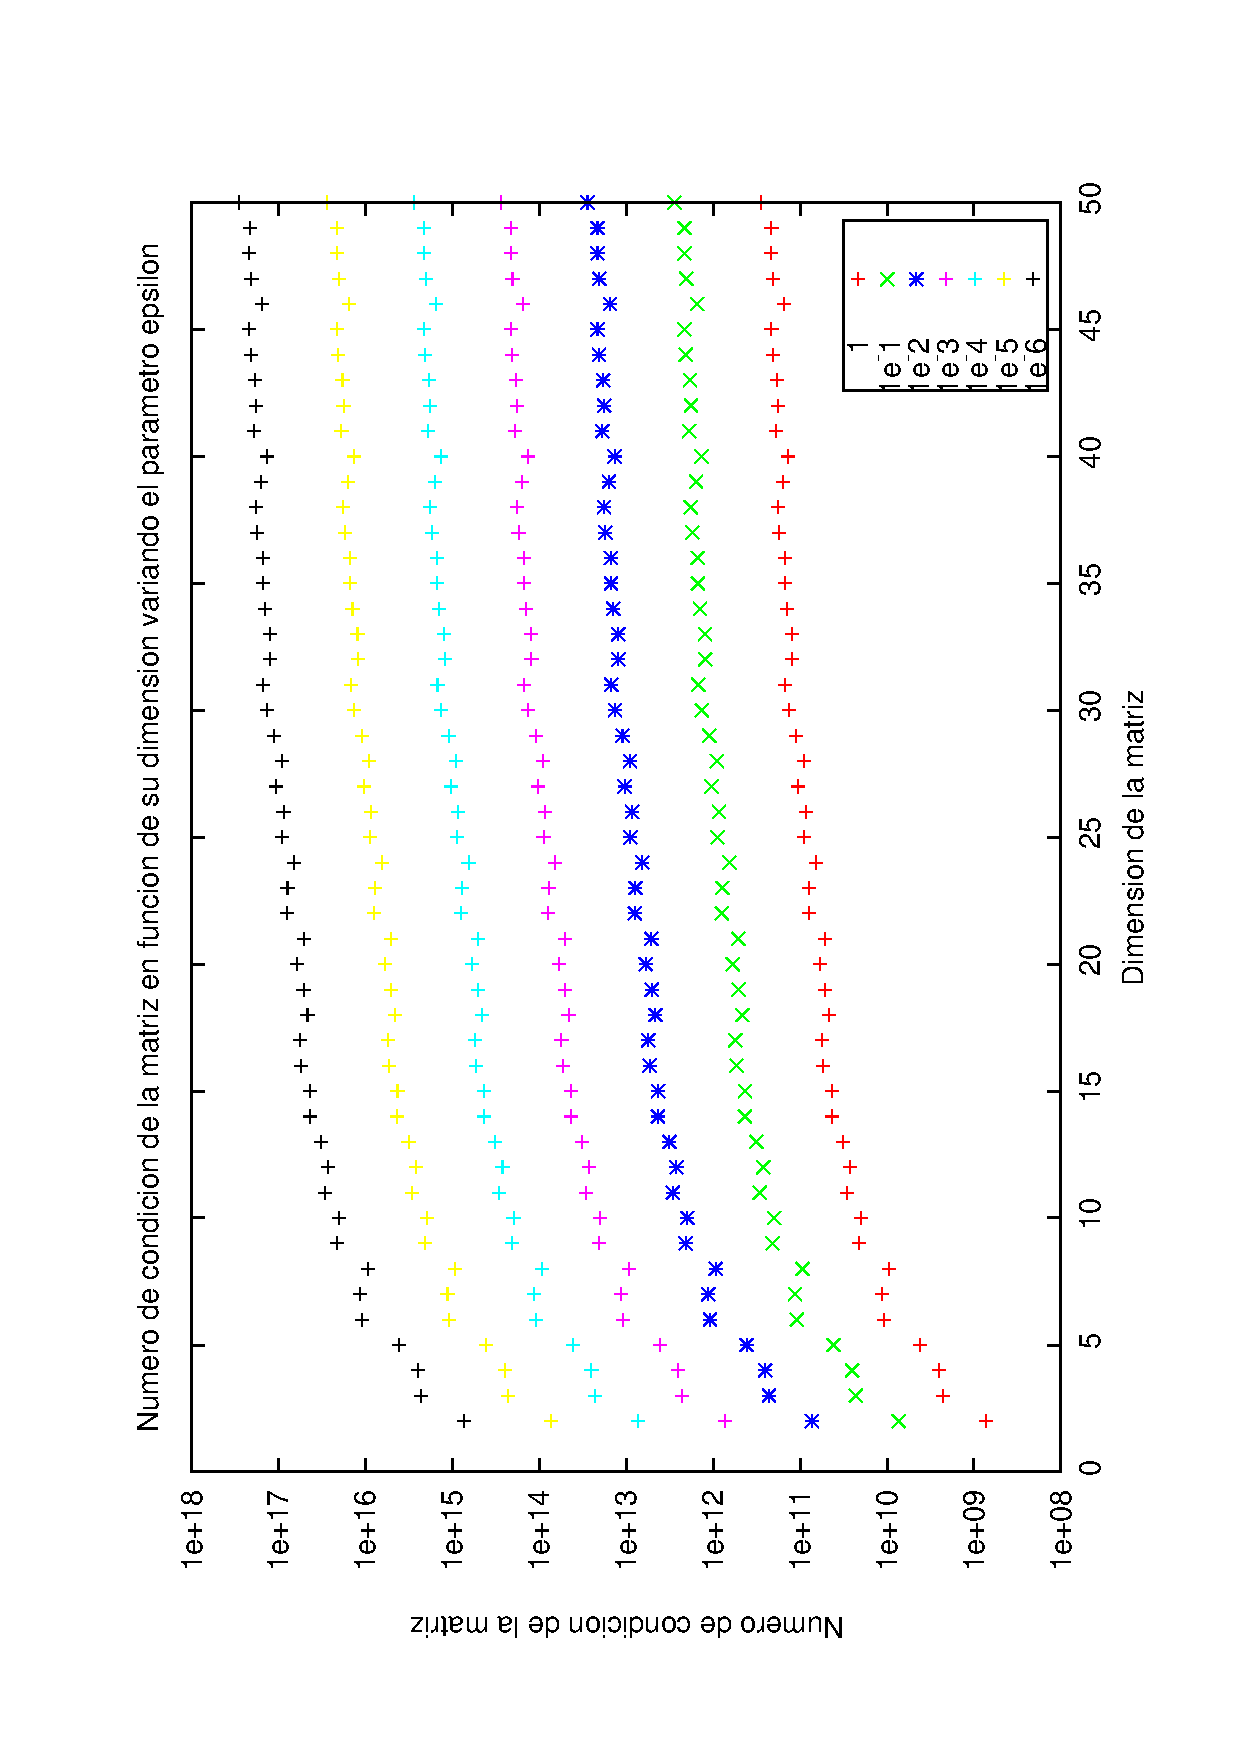
\includegraphics[width=14cm]{graficos/ajuste_epsilon.pdf}
	  \caption{Número de condición de la matriz en función de su dimensión variando el parámetro epsilon}
	  \label{fig:epsilon}
	\end{figure}
	
	\VSP
	
	Para comparar los métodos de resolución de sistemas de ecuaciones lineales implentados (inversa y LU) realizamos el siguiente gráfico que muestra la exactitud de la solución en función de la dimensión de la matriz. Corrimos las pruebas para matrices de dimensión $2$ a dimensión $50$.
	
	Para medir la exactitud de la solución tomamos la norma2 de la diferencia entre la solución calculada y la solución real.
	
	El gráfico se presenta bajo una escala logaritmica en el eje $y$.
	
	\begin{figure}[H]
	  \centering
		\includegraphics[width=14cm]{graficos/inv_vs_lu.pdf}
	  \caption{Distancia a la solución exacta del sistena en funcion de la dimension de la matriz usando el método de la inversa y factorizacion LU}
	  \label{fig:inv_vs_lu}
	\end{figure}
\end{section}

	\newpage
	\begin{section}{Discusión}
	En esta sección, buscaremos conclusiones a la información suministrada por los gráficos de la sección anterior.\\
	
	El primer gráfico presenta la calidad de las matrices mal condicionadas generadas fijando un epsilon (Figura:\ref{fig:epsilon}).
	
	Observamos que a medida que fijamos un $epsilon$ menor, obtenemos una matriz con un número de condición mayor. Más aun, el disminuir un orden de magnitud al $epsilon$ implica un aumento en un orden de magnitud en el número de condición de la matriz.
	
	Este gráfico dio sustento a nuestra hipotesis presentada anteriormente (a menor $epsilon$ mayor número de condición).
	
	A partir del gráfico podemos decir también que cuanto mayor sea la dimensión de la  matriz peor condicionada estará (al menos construyendolas de esta manera) ya que los valores obtenidos (número de condición) en función de la dimensión de la matiz, fijando un $epsilon$, forman una curva logarítmica. Como el gráfico se encuentra bajo una escala logarítmica el número de condición de la matriz crece linealmente conforme aumenta su dimensión.
\end{section}

	\newpage
	\begin{section}{Conclusiones}
	El cálculo sobre aritmética finita presenta un gran desafío para los desarrolladores, al intentar proponer nuevas maneras que minimicen esta pérdida de información, como para quienes utilizan estas herramienta para el cálculo. Si bien hasta el momento no hemos encontrado herramientas que puedan presentar un resultado exacto en todos los casos, conocer como acotar estos errores, nos da una ayuda extra para poder entender a qué corresponde los resultados en la experimentación.

	Inclusive, sabiendo el error cometido en los cálculos, la representación de esta información tanto en gráficos, como en cualquier medio observable de datos, también agrega un margen de error que hay que ser muy precavido que existe, para no llegar a falsas conclusiones.
	
	Existe un factor dominante a la hora de implementar algoritmos o utilizarlos, que es el requerimiento de eficiencia. Los tres algoritmos muestran esta estrecha relación que hay entre precisión y eficiencia. Si bien el tercer algoritmo es el que más rápido aproxima, también su complejidad asíntotica es la mayor (se podría demostrar que es \Ode{n^2}), al igual que $Machin$ y complejidad lineal para $Gregory$. Dependiendo del contexto en el que se utilice, quizás la pérdida de precisión, se justifica por el orden de magnitud de diferencia en el cálculo.\\
	
	Deberíamos tener en cuenta también, que utilizamos como base, los tipos nativos de C++, si necesitamos por ejemplo, mayor precisión, agregamos un nuevo factor que es la cantidad de memoria utilizada, la cual en principio podría no ser acotada.
	
	Encontrar el balance entre estos tres problemas reales es muy complejo, pero herramientas como el cálculo del error relativo, nos ayudan a bislumbrar con mejor claridad, cuál es la mejor opción para cada contexto.\\
	
	Nos han surgido varias implementaciones alternativas, así como desiciones estructurales quizás mejores, equilibrando el tiempo disponible y la complejidad de llevarlas acabo, optamos por esta clase $Real$. Sin embargo, nos gustaría denotar algunas de esas ideas a continuación.
	
	Con respecto a la implementación de los algoritmos, existen funciones que podrían haber sido optimizadas, como el cálculo de la potencia el cual podría haberse implementado de forma más inteligente utilizando programación dinámica, recordando los valores ya calculado para no repetirlos. Podría haberse evitado la generación de un objeto $Real$ por cada iteración de los algoritmos de aproximación a $\pi$.

	Entre alguna de las ideas tratadas en el grupo, surgió lamentablemente cuando el trabajo ya estaba avanzado, la idea de trabajar con fracciones y no reales. Es decir, si consiguiéramos una representacion sin errores para el numerador y denominador (ejemplo, enteros de precisión arbitraria), podríamos realizar todas las cuentas evitando casi toda pérdida de presición (salvo la representación quizás por salida estándar). Si bien, nos interesó muchísimo esta idea, su implementación hubiera sido mucho más compleja, al no poder contar con los algoritmos ya existentes en $doubles$.
	
	La clase $Real$ se implementó de forma tal que acepte la realización de operaciones entre objetos con distinta precisión con el fin de agregar a los resultados diferentes tests como por ejemplo, analizar el impacto de utilizar en el denominador presición mayor a la del numerador, etc. Se implementó además de forma tal que deje al usuario elegir entre truncamiento o redondeo a $t$ bits. Encontramos ciertos casos donde el redondeo no se porta de la forma esperada, y no pudimos corregirlo. Nos parece adecuado igual, dejarlo implementado, con el objeto tanto de presentar el concepto general del programa generado, como no producir quizás imperceptibles errores que compliquen la entrega del trabajo. 

\end{section}

	\newpage
	\begin{section}{Apéndices}
	\begin{subsection}{Apéndice A: Enunciado}
		\parindent = 0 pt
\parskip = 11 pt
\pagestyle{empty}

\newcommand{\real}{\ensuremath{\mathbb{R}}}

%\begin{document}

\begin{centering}
\bf Laboratorio de M\'etodos Num\'ericos - Primer cuatrimestre 2011 \\
Trabajo Pr\'actico N\'umero 2: La Guerra Lineal, Episodio 5 ... \\
\end{centering}

\vskip 25pt
\hrule
\vskip 11pt

{\bf Introducci\'on}

Corr\'ia el a\~no 4957 de la era de paz iniciada luego de la expulsi\'on de los mutantes invasores
en el sistema solar de la estrella HAL-9000 cuando los sistemas de defensa alertaron a la comandancia 
por la intrusi\'on de naves esp\'ias provenientes de lejanas galaxias dominadas por especies hostiles.
Luego de estas primeras incursiones comenzaron los devastadores ataques alien\'igenas. Las fuerzas de 
dicho sistema solar se enfrentaban al ataque de un enemigo muy superior, que amenazaba con
conquistar a todos los planetas del sistema y comenzar as\'i una avanzada sobre la Rep\'ublica
Gal\'actica.

Los sistemas de defensa convencionales pronto fueron insuficientes para resistir el ataque y, adem\'as, 
las inspecciones telem\'etricas dieron cuenta de que, fuera de los l\'imites del sistema solar, el
enemigo estaba ensamblando un Ca\~n\'on Warp, el arma m\'as devastadora jam\'as construida por seres
inteligentes. Los registros de la Rep\'ublica solamente consignaban cuatro ataques previos por
medio de este tipo de armas: en el primer ataque al sistema Z-80\footnote{La Guerra Lineal, 
Episodio 1: TP1 del segundo cuatrimestre de 2000.}, en la batalla de la estrella 80286\footnote
{La Guerra Lineal, Episodio 2: TP2 del primer cuatrimestre de 2001.}, en las guerras de los clones 
de PCs\footnote{La Guerra Lineal, Episodio 3: TP2 del primer cuatrimestre de 2005.}, y en el segundo 
ataque al sistema Z-80\footnote{La Guerra Lineal, Episodio 4: TP2 del segundo cuatrimestre de 2008.}.
La \'unica resistencia posible contra un Ca\~n\'on Warp es utilizar otro Ca\~n\'on Warp, con lo
cual se hizo un llamado desesperado a las fuerzas de l\'inea de la Rep\'ublica para responder a
este ataque. En menos de dos semanas el Ca\~n\'on Warp del Ej\'ercito de la Rep\'ublica estaba
preparado para dar batalla, y el combate decisivo estaba por comenzar...

{\bf La Guerra Lineal}

La batalla entre dos Ca\~nones Warp no es un combate entre bandoleros espaciales, sino una
caballerosa justa algebraica entre dos naves que respetan ciertas reglas. Para
no ser directamente visible, cada nave se sit\'ua en un punto del hiperespacio de $n$ dimensiones.
Llamemos $x \in \real^n$ e $y \in \real^n$ a los puntos donde se ubican la primera y la 
segunda nave, respectivamente.

A intervalos regulares, cada nave realiza un disparo de su Ca\~n\'on Warp con el objetivo de
desintegrar al enemigo. Debido a que nos encontramos en el hiperespacio, la \'unica forma de
dirigir el disparo hacia la posici\'on de la nave enemiga es mediante una transformaci\'on del
espacio--tiempo, llamada \emph{transformaci\'on warp}. Esta transformaci\'on modifica el espacio--tiempo 
de manera tal que la bomba lanzada por la nave en la posici\'on $x$ y sometida a la transformaci\'on warp $A$ ``explotar\'a'' en la posici\'on 
$d = A x$ luego del disparo. Una transformaci\'on warp est\'a dada, entonces, por una matriz \emph{inversible}
$A \in \real^{n \times n}$. La nave enemiga es destruida si y solo si 
$\left\| d - y \right\|_2  \leq 1$. 

Ahora bien, supongamos que la nave $y$ no es destruida. Esta nave puede ver el punto $d$ donde
se produjo la explosi\'on y, analizando las distorsiones del espacio--tiempo sobre el fondo de 
estrellas fijas, tambi\'en puede deducir la transformaci\'on warp $A$ que us\'o el enemigo. 
Entonces, al menos en teor\'ia, puede resolver el sistema $A x = d$ para averiguar la posici\'on 
$x$ del enemigo y eliminarlo en su siguiente disparo. Aqu\'i entra en juego la habilidad de cada 
contendiente para evitar ser f\'acilmente descubierto luego de cada disparo propio, y para descubrir 
la ubicaci\'on del rival luego de cada disparo enemigo.

La Guerra Lineal consiste en una sucesi\'on de disparos simult\'aneos de cada contendiente,
hasta que uno de ellos es destruido (o ambos son destruidos al mismo tiempo). Luego de cada
disparo, cada nave recibe la informaci\'on telem\'etrica de la posici\'on del disparo enemigo y la transformaci\'on
warp que us\'o el adversario, con lo cual podr\'a ajustar su siguiente disparo para acercarse m\'as
a la nave enemiga.

{\bf Detalles y requerimientos}

El objetivo del trabajo pr\'actico es implementar un Control de Ca\~n\'on Warp: un programa que desarrolle autom\'aticamente
una batalla de la Guerra Lineal contra el programa de otro grupo, de acuerdo con las siguientes
especificaciones. 

Cada ejecuci\'on del programa corresponde a un disparo del ca\~n\'on. Cada programa se ejecuta por l\'inea de comandos y toma
como par\'ametros los nombres de varios archivos. Algunos archivos contienen
la posici\'on de la nave y los disparos enemigos, y otro archivo contendr\'a la salida del programa.

Una vez le\'ido el o los archivos de entrada el programa debe seleccionar una transformaci\'on warp $A \in 
\real^{n \times n}$ y realizar un disparo $d = A x$. A partir del segundo turno el programa contar\'a 
con informaci\'on que le permitir\'a inferir la posici\'on del oponente y podr\'a elegir una transformaci\'on
de manera que el disparo se acerque a la nave enemiga. Una vez decidida la transformaci\'on y calculado el disparo
el programa debe informar los mismos en el archivo de salida.

Luego de escribir este archivo, el programa debe detener su ejecuci\'on y ser\'a vuelto a ejecutar
cuando llegue el momento de realizar un nuevo disparo (en el siguiente turno). 
Este proceso contin\'ua hasta que alguno de los dos contendientes es eliminado.
Cualquier
informaci\'on que sea necesario registrar entre disparos se debe almacenar en archivos auxiliares (en el ``directorio actual''),
a criterio del grupo. 

Los programas ser\'an invocados en el primer turno con la siguiente l\'inea de comandos:

\verb|<programa> <posicion> <salida>|

y del segundo turno en adelante, una vez que se cuenta con los datos que gener\'o el programa
rival, ser\'an invocados con la siguiente l\'inea de comandos:

\verb|<programa> <posicion> <salida> <ultimo> <anteriores>|

Por ejemplo:

\verb|lineal.exe datos.txt disparo.txt d001.txt otros.txt|

De acuerdo a los siguientes detalles:
\begin{enumerate}
 \item[programa] Es el programa de cada grupo.
 \item[posicion] Es un archivo con el siguiente formato:
\begin{itemize}
    \item La primera l\'inea contiene un cero\footnote{Por razones hist\'oricas.}.
    \item La segunda l\'inea contiene el valor de $n$, especificando la cantidad de dimensiones del
    espacio en el que se juega.
    \item La tercera l\'inea contiene la posici\'on del jugador, especificada por $n$ valores separados
    por espacios.
\end{itemize}
Por ejemplo, el siguiente es un archivo v\'alido de entrada:
\begin{verbatim}
0
2
-9.51013587206640810000e+001 3.17965084444715660000e+001
\end{verbatim}
\item[salida] Es el archivo que debe generar el programa, conteniendo la transformaci\'on warp elegida y el disparo resultante. Su formato debe ser el siguiente:
\begin{itemize}
    \item La primera l\'inea debe contener el n\'umero del turno en que se efectu\'o el disparo 
    (el primer turno es el n\'umero 1).
    \item La segunda l\'inea debe contener la dimensi\'on $n$ (este valor ya es conocido, pero se incluye
    en el archivo para verificar que no haya inconsistencias).
    \item La tercera l\'inea debe contener las $n$ coordenadas del vector $d$, separadas por espacios.
    \item Las siguientes $n$ l\'ineas contienen los coeficientes de la matriz $A$, ubicando en cada
    l\'inea una fila completa de la matriz (con los coeficientes separados por espacios).
\end{itemize}
\item[ultimo] Contiene el disparo generado por el programa oponente en el turno anterior, con el formato descripto anteriormente.
\item[anteriores] Es una concatenaci\'on de todos los archivos de disparos del oponente, salvo el \'ultimo. En el segundo turno es un archivo vac\'io. En el tercer turno contiene el disparo del turno 1, en el cuarto turno contiene el disparo del turno 1 seguido del disparo del turno 2, etc.
\end{enumerate}



En todo momento el combate estar\'a supervisado por un programa que oficiar\'a de \'arbitro entre
los dos programas en juego (por razones hist\'oricas, este \'arbitro ser\'a llamado La Fuerza),
que se encarga de ejecutar ambos programas y de pasarles como par\'ametros los archivos
que correspondan en cada caso. 

Para asegurar el desarrollo normal de la competencia, el
programa jugador se debe implementar bajo el sistema operativo Windows, de manera 
que sea posible su ejecuci\'on en las m\'aquinas del Laboratorio~6.

El combate debe desarrollarse en aritm\'etica de punto flotante de doble precisi\'on (8 bytes,
correspondiente al tipo de datos \verb|double|). La Fuerza tomar\'a los datos como \verb|doubles|, con lo
cual es importante tomar los recaudos necesarios para la lectura y escritura de los archivos. Todos los archivos generados, tanto por La Fuerza como por los
contrincantes, ser\'an archivos ASCII conteniendo s\'olo n\'umeros, espacios y fin de
l\'inea. Todos los n\'umeros de punto flotante ser\'an escritos usando 20 d\'igitos y
notaci\'on cient\'ifica\footnote{Una opci\'on es \texttt{precision(20)} y
\texttt{setf(std::ios\_base::scientific,std::ios\_base::floatfield)} de
\texttt{std::ostream}. Ejemplo: -1.64741740540787990000e+002 .}, para evitar errores
de representaci\'on.


{\bf Comentarios destacables}

Es importante que el programa implementado cuente con estrategias inteligentes de defensa,
que no le permitan al enemigo deducir f\'acilmente nuestra posici\'on. Por ejemplo, no ser\'ia
muy inteligente utilizar como transformaci\'on warp una matriz diagonal, dado que en este caso el
enemigo puede encontrar nuestra posici\'on con mucha precisi\'on. El informe debe contener
todas las alternativas que el grupo haya considerado con relaci\'on a este punto, junto con una
discusi\'on que justifique la opci\'on finalmente adoptada.
Adem\'as, el informe debe justificar que la matriz generada en cada turno es inversible.
Tambi\'en es importante que el programa est\'e preparado para actuar ante las posibles estrategias de defensa del enemigo. El programa debe contemplar que el enemigo puede estar
generando transformaciones warp que dificulten nuestro an\'alisis de su posici\'on, y debe implementar
alg\'un mecanismo que intente manejar esta situaci\'on.
No
se aceptar\'an transformaciones warp que no sean inversibles, disparos que est\'an mal calculados,
o el uso indebido de espadas l\'aser entre los contrincantes. Recuerden que la Guerra Lineal es
un combate entre caballeros.

\vskip 15pt
\hrule
\vskip 11pt

{\bf Entregas parciales}
\vspace{-15pt}
\begin{description}
  \setlength{\itemsep}{0pt}
  \setlength{\parskip}{0pt}
  \setlength{\parsep}{0pt}
 \item[6 de mayo:] Implementaci\'on del (o de los) m\'etodo(s) de resoluci\'on de sistemas de ecuaciones.
 \item[13 de mayo:] Implementaci\'on completa y casos de prueba.
\end{description}

{\bf Entrega Final}
\vspace{-15pt}
\begin{description}
  \setlength{\itemsep}{0pt}
  \setlength{\parskip}{0pt}
  \setlength{\parsep}{0pt}
 \item[Formato Electr\'onico:] 19 de mayo de 2011, hasta las 23:59 hs, a la direcci\'on: 

  {\emph{metnum.lab2011@gmail.com}}
 \item[Formato f\'isico:] 20 de mayo de 2011, de 17 a 21 hs.
\item[Batalla lineal entre grupos:] 20 de mayo de 2011, de 20 a 21 hs.
\end{description}

%\end{document}


	\end{subsection}
	\begin{subsection}{Apéndice B: Códigos fuente}
	\end{subsection}	
\end{section}

	\newpage
	\begin{section}{Referencias}
	\begin{itemize}
		\item Burden y J.D.Faires, Análisis numérico, International Thomson Editors, 1998
	
		\item http://en.cppreference.com/w/cpp
	\end{itemize}
\end{section}

\end{document}
